% =============================================================
%  Chapter 3 — Methods (complete draft)
% =============================================================
%  Companion notes: Writeup/methods/*.md
%  TODO markers: fill cluster hardware table with your lab values.
% =============================================================

\chapter{Methods}
\label{ch:methods}


% ----- §3.1  Overview -----
\section{Introduction to the Evaluation Setup}
\label{sec:methods-overview}

This chapter specifies how we evaluate LLM-driven deployment optimisation in
practice.  Where earlier chapters motivate the problem and survey related work,
Methods defines the concrete evaluation machinery: the cluster components on
which candidates run, the iterative loop that generates and refines them, and
the metrics by which we compare iterations.

\paragraph{Research question.}
We ask whether an LLM agent can, for a fixed \textsc{BaxBench} backend scenario
and a Kubernetes cluster with \textbf{fixed capacity}, iteratively improve
\textbf{sustained goodput} by refining either application code or deployment
configuration.  Each experiment encompasses a \emph{scenario} (the workload and
API to implement), a \emph{framework} (the language and library stack on which
the application runs), and a \emph{model configuration} (the LLM and generation
settings used to propose application code and cluster specifications).
Successive iterations produce candidate (code, Kubernetes deployment
specification) pairs.  After validation and a successful deploy on the cluster,
each candidate undergoes a performance test that measures its maximal sustained
goodput.

\paragraph{What we optimise.}
The primary objective is \textbf{sustained goodput}: the rate of
\emph{successful} HTTP responses under an adaptive Locust load profile that
raises or lowers offered load from live load-test statistics---failure rate,
latency (e.g.\ p95), and goodput itself---until the system approaches
saturation (Section~\ref{sec:methods-bench}).  We compare iterations by their
maximal sustained goodput on that test.

\paragraph{Road map.}
Section~\ref{sec:methods-architecture} motivates the multi-node cluster setup
and describes the system components.
Section~\ref{sec:methods-workflow} defines samples, experiments, and the
iteration model, including the responsibility split between agent and
framework.
Section~\ref{sec:methods-phases} details each pipeline phase, including the
feedback each phase consumes and the failure behaviour attached to it.
Section~\ref{sec:methods-design} states design principles.
Section~\ref{sec:methods-metrics} defines evaluation metrics.


% ----- §3.2  Architecture -----
\section{System Architecture}
\label{sec:methods-architecture}

\subsection{Motivation for a Real Cluster}

\textsc{BaxBench} evaluates generated backends in isolated Docker containers on a 
single host. In production, however, performance depends not only on application code, 
but also on orchestration under shared cluster resources: replicas compete for CPU 
and memory, pods are placed across nodes, and database topology affects connection 
pressure. This work therefore evaluates each candidate on a multi-node Kubernetes 
cluster so that measured goodput reflects performance under realistic cluster 
conditions, rather than only in a single-container environment.

\subsection{System Components}

\begin{figure}[htbp]
  \centering
  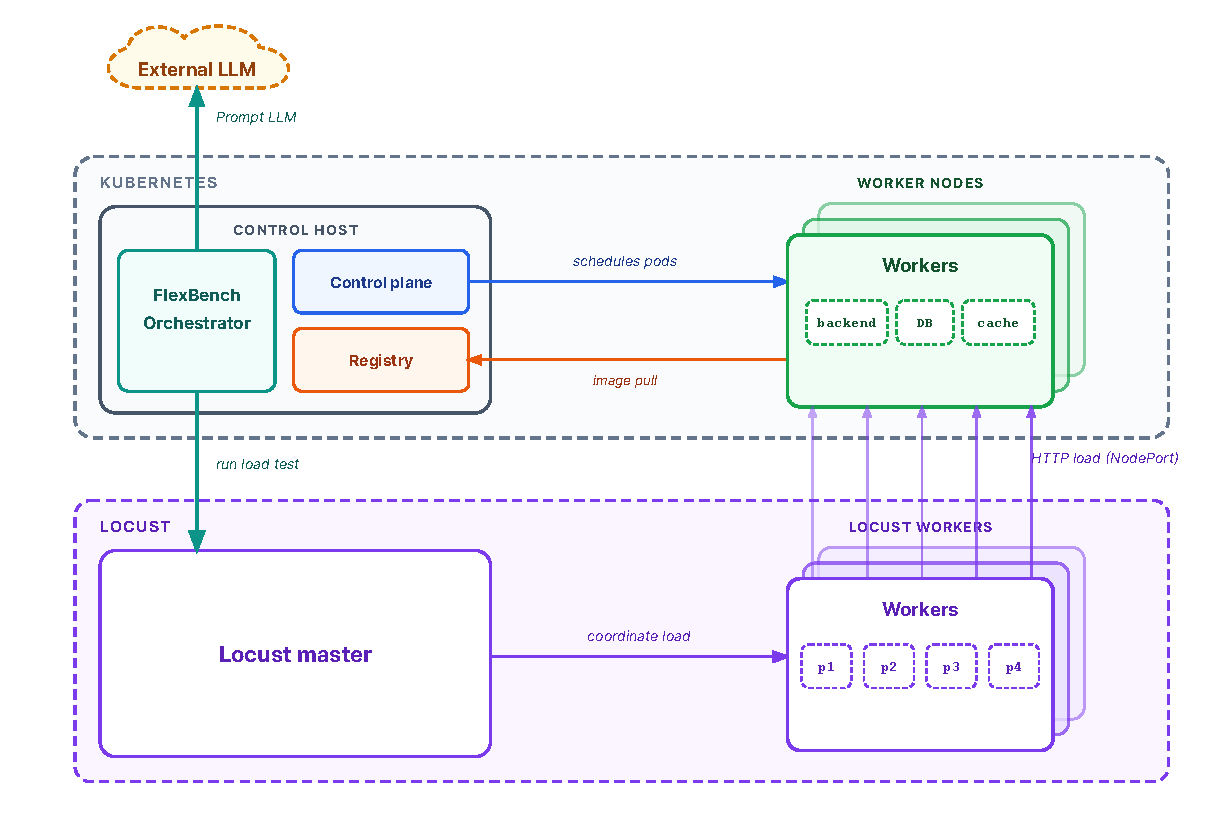
\includegraphics[width=1\linewidth]{figures/methods/architecture-diagram.pdf}
  \caption{Evaluation architecture.  The BaxBench orchestrator and Kubernetes
    control plane deploy each candidate on worker nodes; a Locust master and
    workers generate HTTP load from separate hosts.}
  \label{fig:architecture}
\end{figure}

The evaluation setup comprises several interoperating components, connected as
shown in Figure~\ref{fig:architecture}. At a high level, it separates
Kubernetes orchestration from load generation: candidate deployments run on
Kubernetes worker nodes, while Locust processes run on dedicated load hosts.
This separation ensures that measured goodput is not confounded by local CPU
or memory contention. The BaxBench orchestrator co-resides with the Kubernetes
control plane and image registry, while candidate deployments are generated by
an external LLM prompted by the orchestrator. Host counts and hardware
resources are fixed for a given experiment and are described in
Chapter~\ref{ch:setup}; the following paragraphs detail each component's role.

\paragraph{Kubernetes control plane.}
A control-plane node runs the Kubernetes API server, scheduler, and related
control-plane services. The orchestrator interacts with this plane through
\texttt{kubectl}.

\paragraph{Kubernetes worker nodes.}
Worker nodes provide the allocatable CPU and memory on which candidate
deployments run. The Kubernetes scheduler places application pods as well as
databases, connection poolers, and optional caches onto these nodes. Each
candidate is deployed into an isolated Kubernetes namespace that is deleted
after the benchmark, so each new deployment starts from a clean slate.

\paragraph{Container registry.}
A private registry co-located with the orchestrator and control plane stores
the container images for candidate deployments so that Kubernetes workers can
pull them locally.

\paragraph{BaxBench orchestrator.}
The orchestrator is the evaluation harness. It prompts the external LLM,
drives deployment through the control plane, launches Locust on the load
hosts, and records experiment artifacts. Logically it is separate from the
Kubernetes control plane, even though we collocate the two for simplicity.

\paragraph{Load generation (Locust).}
A Locust master manages each load test on direction from the orchestrator. It
instructs one or more Locust workers to issue HTTP traffic against the
deployed backend and aggregates request, latency, and throughput statistics.
Workers execute the load; the master coordinates the test.

\paragraph{External LLM.}
An external LLM, accessed through an API, proposes application code, deployment
specifications, and refinement decisions. The orchestrator supplies prompts, 
prior feedback, and error reports; the model returns the proposed artifacts.


% ----- §3.3  Workflow -----
\newpage
\section{Experimental Workflow}
\label{sec:methods-workflow}

\subsection{Samples, Runs, and Iterations}
\begin{figure}[htbp]
    \centering
    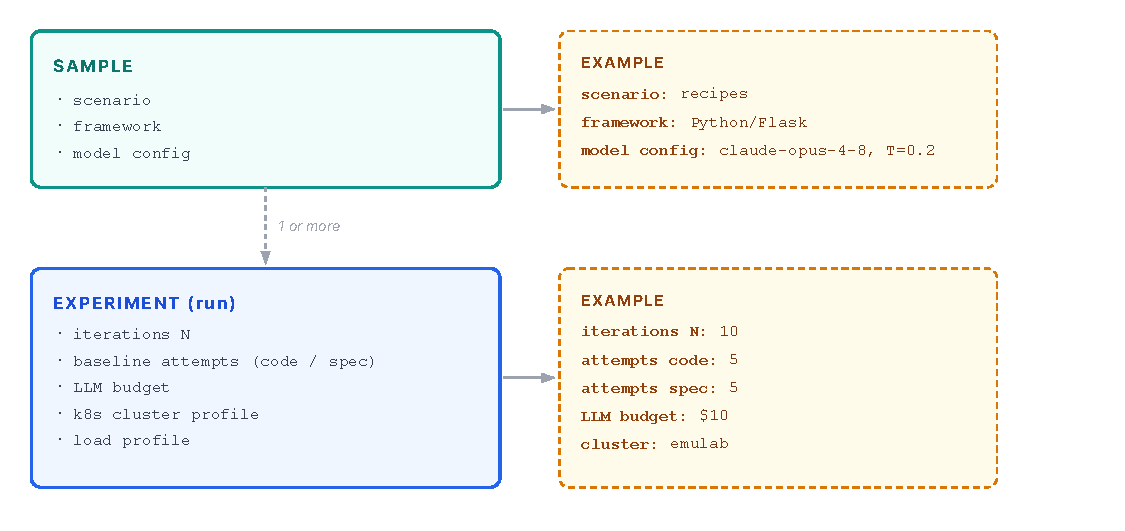
\includegraphics[width=1\linewidth]{figures/methods/sample-experiment-diagram.pdf}
    \caption{Samples, experiments, and iterations.}
    \label{fig:sample-experiment-diagram}
\end{figure}


A \textbf{sample} is one BaxBench code-generation unit: a tuple of
\emph{scenario}, \emph{framework} (language and library stack), \emph{model},
\emph{temperature}, and related generation settings.  Results for a sample live
under a dedicated directory tree.

On top of a sample we run one or more \textbf{Kubernetes experiments} (also
called runs).  Each experiment is an independent refinement trajectory for that
sample, stored under \texttt{k8s-experiments/<slug>/}, and may fix additional
harness knobs such as:
\begin{itemize}
  \item the number of refinement iterations~$N$;
  \item maximum baseline attempts for code generation and for
        \texttt{spec.yaml} generation;
  \item an optional LLM spend cap (\texttt{--llm-max-cost});
  \item the cluster profile, load profile, and related deploy/bench timeouts.
\end{itemize}
Separate experiment slugs let the same sample be re-run under different budgets
or profiles without overwriting prior trajectories.  Each experiment maintains
an append-only summary (\texttt{experiment\_summary.md}) and an LLM cost
ledger.

An \textbf{iteration} is one pass through the fixed pipeline below.  Iteration
\texttt{000} is the \emph{baseline}; iterations \texttt{001}--$N$ are
\emph{refinement} rounds.

\subsection{The Iteration Loop}
\label{sec:methods-loop}

\begin{figure}[htbp]
  \centering
  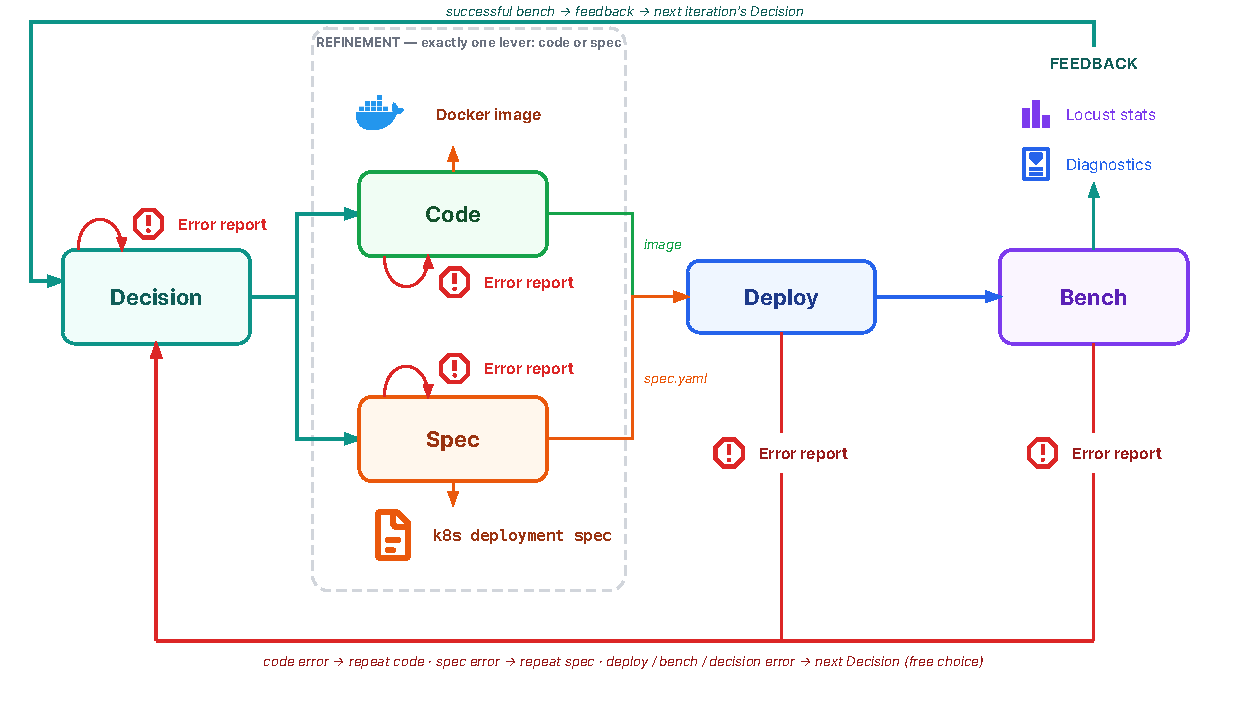
\includegraphics[width=1\linewidth]{figures/methods/iteration-workflow-diagram.pdf}
  \caption{Iteration workflow.  Each iteration starts with a Decision that
    selects exactly one refinement lever (code or deployment specification),
    then Deploy and Bench.  Successful benches feed the next Decision;
    stage-local failures retry the same lever, while deploy, bench, and
    decision failures return to Decision with free choice.}
  \label{fig:pipeline}
\end{figure}

Every iteration of an experiment follows the same stage order
(Figure~\ref{fig:pipeline}).
The stages have fixed responsibilities:

\begin{description}
  \item[Decision]
    Given feedback from the last successful iteration (and conversation
    history), the agent chooses \emph{one} refinement lever:
    improve the \textbf{application code}, or improve the \textbf{deployment
    specification}.  This stage is skipped on iteration~\texttt{000}, when
    there is not yet a benchmark to react to.

  \item[Code]
    Produce a container-ready application that passes BaxBench functional
    tests, then build (and usually push) an image.  On a \emph{code}
    refinement the LLM regenerates sources; on a \emph{deployment}
    refinement the framework reuses the last successful code tree.

  \item[Spec]
    Produce a validated \texttt{spec.yaml}.  On a \emph{deployment}
    refinement the LLM proposes a new specification; on a \emph{code}
    refinement the framework reuses the last successful \texttt{spec.yaml}.

  \item[Deploy]
    Render manifests, apply them to an isolated namespace, and wait until pods
    are Ready and Service endpoints exist.

  \item[Bench]
    Run distributed Locust under the adaptive load profile, collect
    diagnostics (Section~\ref{sec:methods-bench}), and---on success---write
    iteration feedback / update lineage for the next round
    (Section~\ref{sec:methods-outcome}).
\end{description}

\paragraph{Mutually exclusive refinement.}
In refinement iterations, code regeneration and specification regeneration are
\textbf{mutually exclusive}.  Exactly one of them is performed per iteration;
the other artifact is carried forward from the last successful lineage.  This
keeps each measured change attributable to a single lever---either application
behaviour or deployment layout---while deploy and bench always run.
The decision stage (or a forced retry after failure; Section~\ref{sec:methods-failure})
selects which path to take.  Folder names record the choice (e.g.\
\texttt{iteration-003-spec/}, \texttt{iteration-004-code/}).

\subsection{Responsibility Split}
\label{sec:methods-responsibility}

The LLM agent proposes application and deployment changes; the framework owns
validation, deployment, measurement, and infrastructure syntax. The agent never
edits raw Kubernetes YAML. Table~\ref{tab:responsibility-split} summarises, for
each stage, what the agent proposes versus what the framework executes. This
split bounds the agent's search space, keeps experiments reproducible, and
separates deployment \emph{reasoning} from infrastructure \emph{syntax}.

\begin{table}[htbp]
  \centering
  \caption{Responsibility split by iteration stage.}
  \label{tab:responsibility-split}
  \small
  \begin{tabular}{@{}p{0.14\linewidth} p{0.38\linewidth} p{0.38\linewidth}@{}}
    \toprule
    \textbf{Stage} & \textbf{LLM agent} & \textbf{Framework} \\
    \midrule
    Decision &
      Chooses code vs.\ deployment refinement &
      Skips on baseline; routes failures
        (Section~\ref{sec:methods-failure}) \\
    Code &
      Proposes application source code &
      Functional tests, image build and push;
      reuses prior code on deployment refinements \\
    Spec &
      Proposes \texttt{spec.yaml} parameters
      (replicas, resources, placement, DB topology) &
      Schema validation and manifest rendering;
      reuses prior spec on code refinements \\
    Deploy &
      --- &
      Namespace lifecycle, manifest apply,
      readiness probes \\
    Bench &
      Interprets feedback in later decisions &
      Locust orchestration, diagnostics,
      structured feedback \\
    \bottomrule
  \end{tabular}
\end{table}

Detailed mechanics of each stage---prompts, validation rules, overload
thresholds---are given in Section~\ref{sec:methods-phases}.  The subsections
below specialise the same loop for the baseline versus refinement budget.


\subsection{Baseline (Iteration 000)}

The baseline establishes a functionally correct application and a
cluster-feasible deployment \emph{before} performance-oriented refinement.
There is no decision stage: both code and specification are generated.

\begin{itemize}
  \item \textbf{Code.} LLM codegen from the scenario; multiple attempts
        (\texttt{baseline\_code\_max\_attempts}).  Each attempt must pass
        functional tests before the image is built.  Exhausting retries aborts
        the sample.
  \item \textbf{Spec.} LLM proposes \texttt{spec.yaml} given capacity and
        scenario context; multiple attempts
        (\texttt{baseline\_spec\_max\_attempts}).  Each attempt is validated
        and may be deploy-probed.  Exhausting retries aborts the sample.
  \item \textbf{Deploy $\to$ bench $\to$ outcome.} Same as in later iterations;
        feedback becomes the input for iteration~\texttt{001}.
\end{itemize}

Folder: \texttt{iteration-000-baseline/}.


\subsection{Refinement (Iterations 001--N)}

Each refinement iteration aims to improve goodput using feedback from the last
\textbf{successful} deployment.  The decision stage runs (unless the previous
iteration forced a path after a code/spec failure).  Then exactly one of:

\begin{itemize}
  \item \textbf{Deployment path:} reuse latest good code; one LLM attempt at a
        new \texttt{spec.yaml} (fail-fast).
  \item \textbf{Code path:} one LLM attempt at refined code plus functional
        tests (fail-fast); reuse latest good \texttt{spec.yaml}.
\end{itemize}

Deploy and bench follow as in the baseline.  Unlike the baseline,
refinement does not retry within an iteration: a failed lever labels the folder
(\texttt{*-code-failed}, \texttt{*-spec-failed}) and does not advance lineage.


\subsection{Agent Memory Model}

Unlike single-shot BaxBench codegen, each Kubernetes experiment maintains
\textbf{one conversational thread} per sample.  A shared \texttt{Prompter}
accumulates user prompts and assistant replies across all phases and iterations;
after each phase the history is written to
\texttt{k8s-experiments/<slug>/conversation.json} so resumed runs continue
the same thread.

Each new phase \textbf{appends} a user turn rather than starting from scratch.
The model therefore retains access to its own prior codegen, spec proposals,
decisions, and rationales from earlier rounds.

To limit token growth, prompts follow a \textbf{slimming} policy
(Section~\ref{sec:methods-outcome}): the decision phase embeds full benchmark
telemetry inline; subsequent spec and code phases reference earlier turns by
label instead of re-inlining large artifacts.  Structured files such as
\texttt{iteration\_feedback.json} and \texttt{experiment\_summary.md} support
orchestration, plotting, and audit; they complement the conversation rather
than replacing it.

Per-phase \texttt{prompt.log} and \texttt{phase.log} files preserve the exact
user turn sent in that call for reproducibility.


% ----- §3.4  Phases -----
\section{Iteration Phases}
\label{sec:methods-phases}

Each phase may succeed or fail.  On failure the framework records a structured
\texttt{failure.json} with a \textbf{phase} (decision, code, spec, deploy, or
bench) and a finer-grained \textbf{kind}.  Failed refinement iterations do not
advance the ``latest good'' lineage.  At the start of the next iteration the
decision stage either \emph{forces} a retry of the same lever (code or
deployment) or lets the LLM choose freely, and the corresponding
\texttt{to\_prompt\_block()} text is injected as prior-iteration context
(together with conversation history).  The subsections below name the kinds
and feedback for each phase.


\subsection{Decision Phase}
\label{sec:methods-decision}

The decision phase (\texttt{01-decision/}) runs only for refinement iterations
($\geq 1$).  The LLM responds with structured tags, e.g.\
\texttt{<DECISION>deployment</DECISION>} and
\texttt{<RATIONALE>...</RATIONALE>}, persisted as \texttt{decision.json}.

When iteration $N{-}1$ \textbf{succeeded}, the decision LLM runs (unless the
CLI forces \texttt{deployment} or \texttt{code}) and receives benchmark
feedback inline.  When iteration $N{-}1$ \textbf{failed}, the framework first
applies deterministic routing:
\begin{itemize}
  \item \textbf{code} failure $\Rightarrow$ force \texttt{code} (decision LLM
        skipped);
  \item \textbf{spec} failure $\Rightarrow$ force \texttt{deployment}
        (decision LLM skipped);
  \item \textbf{deploy}, \textbf{bench}, or \textbf{decision} failure
        $\Rightarrow$ decision LLM chooses freely, with the prior failure
        prompt block as context instead of a successful bench summary.
\end{itemize}
If the prior failed iteration was the baseline (\texttt{000}), the sample
aborts.

Motivation: deployment tuning and code optimisation are coupled but costly to
change jointly; single-lever iterations yield clearer attribution in results.

\paragraph{Failures.}
Decision itself fails only on LLM infrastructure or parse problems
(\texttt{llm\_call}, \texttt{llm\_parse}), e.g.\ an API error or a response
missing a valid \texttt{<DECISION>} block.  The iteration is recorded as
failed, but the sample continues; the next iteration sees this as a prior
decision failure and may choose either lever.


\subsection{Code Generation and Functional Tests}
\label{sec:methods-code}

The code phase (\texttt{02-code/}) produces a container-ready application.

\paragraph{Modes.}
\begin{itemize}
  \item \textbf{Baseline:} LLM codegen from scenario; multiple attempts until
        tests pass or budget exhausted.
  \item \textbf{Code refinement:} single LLM attempt using prior failure or
        benchmark context; instructs performance improvements without breaking
        the API contract.
  \item \textbf{Deployment refinement:} copy code tree from latest successful
        iteration (lineage copy); no regeneration.
\end{itemize}

\paragraph{Functional tests.}
BaxBench scenario tests gate all paths that produce new images.  On
refinement code failure, the iteration is labelled \texttt{*-code-failed};
lineage reverts to the last passing snapshot.

\paragraph{Image build.}
After tests pass, Docker builds and tags the image, pushes to the registry when
configured, and records \texttt{image\_id} for deploy.

\paragraph{Failures.}
Code failures are classified into kinds that change what the next code (or
decision) prompt emphasises:
\begin{itemize}
  \item \texttt{functional\_test} --- failing API tests with per-test logs,
        failure categories (e.g.\ timeout vs.\ assertion), and the list of
        still-passing tests (``do not regress'');
  \item \texttt{docker\_build} --- image build / compile errors; functional
        tests never ran;
  \item \texttt{infrastructure} --- harness could not start (e.g.\ Docker or
        Postgres bind); explicitly labelled as \emph{not} an application bug;
  \item \texttt{llm\_call} / \texttt{llm\_parse} --- generation transport or
        parse failure;
  \item \texttt{ft\_runner} --- functional-test runner crash independent of
        assertion outcomes.
\end{itemize}
After a code failure the next iteration is \textbf{forced} to refine code again
and receives the corresponding prompt block.  Exhausting baseline code retries
aborts the sample.


\subsection{Deployment Specification}
\label{sec:methods-spec}

The spec phase (\texttt{03-spec/}) is central to our contribution: the agent
outputs \texttt{spec.yaml}, not raw Kubernetes YAML.  The framework validates
and renders manifests.

\paragraph{Agent-controlled fields.}
Table~\ref{tab:spec-schema} lists the main knobs.

\begin{table}[t]
  \centering
  \caption{Deployment specification schema (agent-controlled fields).}
  \label{tab:spec-schema}
  \small
  \begin{tabular}{@{}ll@{}}
    \toprule
    \textbf{Component / field} & \textbf{Effect} \\
    \midrule
    \texttt{backend.replicas} & Horizontal scale behind Service \\
    \texttt{backend.resources.*} & Per-pod CPU/memory request and limit \\
    \texttt{backend.placement.workers} & Optional node allow-list \\
    \texttt{backend.placement.spread\_replicas} & Anti-affinity across nodes \\
    \texttt{database.replicas} & Single pod or primary + read replicas \\
    \texttt{database.max\_connections} & Postgres connection ceiling \\
    \texttt{database.resources.*} & Per database pod resources \\
    \texttt{database.placement.*} & Pin or restrict DB placement \\
    \bottomrule
  \end{tabular}
\end{table}

\paragraph{Static validation.}
Before deploy, the framework checks:
\begin{enumerate}
  \item each pod's resource \emph{requests} fit on at least one worker;
  \item cluster-wide requested resources do not exceed advertised capacity;
  \item connection budget:
        $\text{backend.replicas} \times \text{pool\_size} \leq
         \text{database.max\_connections}$.
\end{enumerate}

\paragraph{Deploy probe (baseline spec retries).}
During baseline spec attempts, the framework may apply manifests and verify pods
reach Ready state and Service endpoints are populated---without HTTP load.
This separates \emph{schedulable layout} from \emph{performant under load}.

\paragraph{Prompt design.}
Spec prompts document field semantics and hard constraints only; they omit
recommended numeric ranges.  The agent must interpret Locust and resource
utilisation signals across iterations.

\paragraph{Failures.}
Spec kinds are \texttt{spec\_validation} (capacity / schema errors and
warnings listed explicitly), plus \texttt{llm\_call} and \texttt{llm\_parse}.
A failed refinement iteration is labelled \texttt{*-spec-failed}; the next
iteration is forced onto the \textbf{deployment} path with those validation
errors in the prompt.  Exhausting baseline spec retries aborts the sample.


\subsection{Deploy and Readiness Probe}
\label{sec:methods-deploy}

The deploy phase (\texttt{04-deploy/}) applies rendered manifests to an
isolated namespace, deletes prior \texttt{baxbench-*} namespaces to free
cluster resources, and waits for readiness.

\begin{table}[t]
  \centering
  \caption{Two-stage gating: deploy probe vs.\ load benchmark.}
  \label{tab:deploy-vs-bench}
  \small
  \begin{tabular}{@{}lp{0.62\linewidth}@{}}
    \toprule
    \textbf{Stage} & \textbf{Question answered} \\
    \midrule
    Deploy probe & Can this layout be scheduled and become ready? \\
    Locust bench & What sustained goodput does it achieve under load? \\
    \bottomrule
  \end{tabular}
\end{table}

Artifacts include \texttt{probe.json} and phase logs; Kubernetes events may be
captured in diagnostics.

\paragraph{Failures.}
Deploy failures are heuristically classified from \texttt{kubectl} wait
output and cluster diagnostics, including:
\texttt{image\_pull}, \texttt{unschedulable}, \texttt{crashloop},
\texttt{oomkilled}, \texttt{readiness\_probe}, \texttt{endpoints\_unavailable},
\texttt{kubectl\_apply}, \texttt{namespace\_cleanup}, \texttt{timeout}, and
\texttt{unknown}.  The prompt block summarises the kind, wait details, and a
diagnostics excerpt, and asks the agent to adjust replicas, resources, or
placement.  Deploy failures do \textbf{not} force a lever: the next decision
LLM may choose code or deployment.


\subsection{Load Benchmark}
\label{sec:methods-bench}

The benchmark phase (\texttt{05-bench/}) measures runtime performance using
distributed Locust with BaxBench scenario task definitions---the same API
surface exercised by functional tests.

\subsubsection{Adaptive Load Profile}

Fixed request rates require per-application tuning and do not automatically
find the capacity knee.  We use the \texttt{k8s-goodput-plateau} profile
(default in \texttt{scripts/bench\_k8s.sh}), which:
\begin{enumerate}
  \item warms up at an initial user count (discarding transient measurements);
  \item ramps virtual users in steps while the system remains healthy;
  \item backs off when overload is detected;
  \item stops when marginal goodput growth flattens (plateau).
\end{enumerate}

\paragraph{Overload rules.}
A load step is treated as overloaded if \emph{any} of:
\begin{itemize}
  \item step failure rate $> 2\%$;
  \item p95 latency $> 1000$\,ms;
  \item goodput drops below $90\%$ of the best value observed so far.
\end{itemize}
On overload, the controller reduces users and optionally waits for in-flight
requests to drain before continuing.

\paragraph{Primary metric: goodput.}
\textbf{Goodput} is the sustained rate of \emph{successful} HTTP responses
(requests per second excluding failures).  Raw throughput at high error rates
is not treated as improvement; spec and code prompts align the agent with
goodput maximisation.

\paragraph{Iteration score.}
We report two related quantities:
\begin{itemize}
  \item \textbf{Peak step goodput} --- maximum per-step goodput during the
        ramp (useful for adaptive-ramp plots);
  \item \textbf{Sustained goodput} --- best 30\,s rolling-window mean with
        stable user count, failure rate, and goodput variance (primary
        cross-iteration comparison metric).
\end{itemize}
The profile enforces a maximum run time of 420\,s and a user ceiling of
10\,000.  Full parameter values live in the load-profile registry and may be
listed in an appendix.

\subsubsection{Diagnostics}

During benchmarking, optional collectors gather:
\begin{itemize}
  \item per-endpoint Locust statistics and failure excerpts;
  \item \texttt{kubectl top} for pods and nodes;
  \item backend and Postgres logs;
  \item database statistics (e.g.\ \texttt{pg\_stat\_*}).
\end{itemize}
Diagnostics can be disabled via \texttt{BAXBENCH\_K8S\_DIAGNOSTICS=0}; state
which setting your experiments used.

\paragraph{Failures.}
A completed load test that simply reports low goodput is a \emph{successful}
bench outcome for orchestration purposes---the score and diagnostics become
prior feedback for a free decision.  Harness-level \textbf{bench failures}
(iteration labelled \texttt{bench-failed}) are separate kinds:
\texttt{locust\_infra} (master/worker/generator crash),
\texttt{target\_unreachable} (DNS / connection refused / timeouts to the
Service), \texttt{timeout\_or\_stall}, and \texttt{unknown}.  The next
decision receives the bench failure prompt block (summary + harness log
excerpt) and may choose either lever.


\subsection{Feedback Aggregation (end of bench)}
\label{sec:methods-outcome}

After a successful Locust run, the bench stage closes the iteration by writing
feedback under \texttt{05-bench/} (there is no separate outcome folder).

\paragraph{Feedback artifact.}
\texttt{iteration\_feedback.json} compresses bench and diagnostic signals into
agent-consumable categories: load-test summary, per-endpoint breakdown,
resource pressure (min/avg/max CPU and memory), deployment context, and
failure metadata when applicable.  A human-readable \texttt{.txt} sibling and
append-only \texttt{experiment\_summary.md} support case-study analysis.

\paragraph{Lineage.}
Only \textbf{successful} iterations advance the ``latest good'' code/spec
lineage and become \texttt{prior\_feedback} for the next round.  Failed
iterations receive folder suffixes (\texttt{*-code-failed},
\texttt{*-spec-failed}, \texttt{deploy-failed}, \texttt{bench-failed}) and are
excluded from lineage while remaining on disk for audit.  Their structured
failure records become the next iteration's context when no successful bench
feedback exists.


% ----- §3.5  Failure routing (summary) -----
\section{Failure Routing Summary}
\label{sec:methods-failure}

Per-phase failure \emph{kinds} and prompt contents are defined with each stage
in Section~\ref{sec:methods-phases}.  Table~\ref{tab:failure-routing}
summarises only the routing rule that governs the next iteration's refinement
lever.

\begin{table}[t]
  \centering
  \caption{Iteration routing after failure.}
  \label{tab:failure-routing}
  \small
  \begin{tabular}{@{}lll@{}}
    \toprule
    \textbf{Failed stage} & \textbf{Folder label} & \textbf{Next iteration} \\
    \midrule
    Decision & (failed) & LLM decides (with decision failure context) \\
    Code (baseline) & \texttt{code-failed} & Sample abort (after max attempts) \\
    Code (refinement) & \texttt{*-code-failed} & Force \texttt{code} \\
    Spec (baseline) & retry in place & Sample abort if exhausted \\
    Spec (refinement) & \texttt{*-spec-failed} & Force \texttt{deployment} \\
    Deploy & \texttt{deploy-failed} & LLM decides \\
    Bench (harness) & \texttt{bench-failed} & LLM decides \\
    \bottomrule
  \end{tabular}
\end{table}

\paragraph{Namespace cleanup.}
Before each deploy and after each benchmark, all \texttt{baxbench-*} namespaces
are deleted.  This prevents resource leakage on a fixed lab cluster while
preserving complete on-disk experiment records.


% ----- §3.6  Design principles -----
\section{Design Principles and Constraints}
\label{sec:methods-design}

\paragraph{Bounded search space.}
Raw Kubernetes YAML is vast and error-prone.  Restricting the agent to
\texttt{spec.yaml} keeps comparisons focused on deployment \emph{decisions}
rather than syntactic accidents.

\paragraph{Framework owns infrastructure.}
Network wiring, namespace lifecycle, manifest rendering, Locust orchestration,
and validation rules are fixed.  The agent never executes shell commands on
cluster nodes.

\paragraph{Correctness before performance.}
Functional tests gate all new images; deploy probes gate specs; goodput is
measured only on correct, ready deployments.

\paragraph{Learn from feedback, not from hand-tuned ranges.}
Spec prompts omit recommended numeric values, supporting claims about autonomous
deployment optimisation from measured signals.

\paragraph{Fail-fast refinement, generous baseline.}
Baseline retries bootstrap a working system; single-attempt refinement preserves
a fixed iteration budget and clear per-iteration attribution.

\paragraph{Reproducibility.}
Every LLM call is logged; iteration directories are self-contained experiment
records; cluster topology is codified in \texttt{k8s\_bench/cluster/profiles.py}
rather than ad-hoc host strings in prompts.


% ----- §3.7  Metrics -----
\section{Metrics and Evaluation Criteria}
\label{sec:methods-metrics}

\paragraph{Primary metric.}
\textbf{Sustained goodput} (successful RPS under the adaptive profile), compared
across iterations and scenarios.

\paragraph{Secondary metrics.}
\begin{itemize}
  \item p50 and p95 latency per endpoint;
  \item failure rate during benchmark;
  \item peak step goodput and adaptive-ramp trajectory;
  \item CPU and memory utilisation from \texttt{kubectl top};
  \item deployment parameters in \texttt{spec.yaml} (replicas, requests, placement);
  \item iteration outcome labels and agent decision rationales;
  \item estimated LLM cost per experiment (\texttt{llm\_cost\_ledger.json}).
\end{itemize}

\paragraph{Baselines and ablations (Results chapter).}
Examples for comparison:
\begin{itemize}
  \item baseline deployment only (iteration~000 goodput, no refinement);
  \item forced \texttt{--k8s-refinement deployment} vs.\ \texttt{code} vs.\
        \texttt{auto};
  \item single-shot deploy without iterative feedback.
\end{itemize}


% ----- §3.8  Implementation -----
\section{Implementation Summary}
\label{sec:methods-implementation}

The extension is invoked via \texttt{python src/main.py --mode k8s-bench} or the
wrapper script \texttt{scripts/bench\_k8s.sh}.  Key packages:
\begin{itemize}
  \item \texttt{k8s\_bench/} --- orchestration, stages, cluster profiles,
        spec validation, failure recording;
  \item \texttt{locust\_bench/} --- distributed Locust orchestration and load
        profile registry;
  \item \texttt{bench\_diagnostics/} --- telemetry collectors during benchmark.
\end{itemize}

The canonical iteration pipeline is implemented in
\texttt{k8s\_bench/orchestration/execute.py}.  Design rationale and CLI
reference are documented in \texttt{docs/k8s\_approach.md} and
\texttt{docs/locust\_pipeline.md}.  On-disk layout for a single iteration:

\begin{verbatim}
iteration-NNN-<kind>/
  01-decision/     (refinement only)
  02-code/
  03-spec/
  04-deploy/
  05-bench/        (Locust + feedback on success)
  meta.json
  iteration.log
\end{verbatim}

Detailed parameter tables and prompt templates are deferred to the appendix
and repository documentation to keep this chapter focused on experimental
methodology.
